\documentclass[aspectratio=1610]{beamer}
\usepackage{graphicx}
\usepackage{amssymb,amsmath,amsfonts}
\usepackage[spanish,es-tabla]{babel}
\usepackage[ansinew]{inputenc}

\usetheme{Madrid} % Cambia "Madrid" por el tema que prefieras
\usecolortheme{default} % Cambia "beaver" por el esquema de colores que prefieras
\usepackage{xcolor}
\setbeamercolor{structure}{fg=green!60!black} % Color principal a un tono de verde
\setbeamercolor{title}{fg=green!60!black} % Establece el color del t�tulo al verde
\setbeamercolor{subtitle}{fg=green!50!black} % Establece el color del subt�tulo al verde

% Ajustes adicionales
\usefonttheme[onlymath]{serif} % Cambiar a fuente serif para matem�ticas



\title{\bf Regresi�n Lineal}
\subtitle{Algunos consideraciones para el an�lisis de datos en los cursos de laboratorio de F�sica}
\author{H�ctor F. Hern�ndez G.}
\date{\today}

\begin{document}

\begin{frame}
    \centering
    \vspace{1cm} % Espacio superior
    {\huge \color{green!60!black}  \inserttitle\par} % T�tulo
        \vspace{0.5cm} % Espacio entre el t�tulo y el subt�tulo
    {\large \color{green!50!black} \insertsubtitle\par} % Subt�tulo en verde
    \vspace{1cm} % Espacio entre el t�tulo y la imagen
    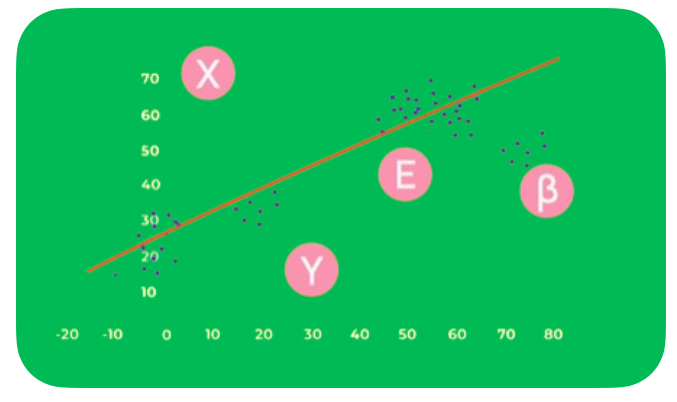
\includegraphics[width=0.7\textwidth]{figuras/fig01} % Imagen
%    \vspace{1cm} % Espacio entre la imagen y el autor
%    {\large \insertauthor\par} % Autor
%    \vspace{0.5cm} \\ % Espacio entre el autor y la fecha 
 %   \insertdate % Fecha
\end{frame}

%\frame{\titlepage}

\begin{frame}
    \frametitle{Regresi�n Lineal}
    \begin{enumerate}
        \item El problema de la regresi�n lineal
        \item La regresi�n lineal simple
        \item M�todo de m�nimos cuadrados
        \item Coeficiente de regresi�n
	\item Coeficiente de correlaci�n lineal
	\item El contraste de regresi�n
	\item Inferencias acerca de los par�metros
	 \item Inferencias acerca de la predicci�n
	 \item Los supuestos del modelo de regresi�n lineal
	\item Un ejemplo en donde no se cumplen los supuestos
    \end{enumerate}
\end{frame}


\begin{frame}
    \frametitle{ El problema de la regresi�n lineal}
    \begin{itemize}
     \item El an�lisis de regresi�n es una t�cnica estad�stica para investigar y modelar relaciones entre variables.
\item Las relaciones estad�sticas difieren de las funcionales porque no son perfectas; las observaciones no caen directamente sobre una curva.
\item Se supone una relaci�n entre una respuesta cuantitativa $y$ y $k$ predictores $x_1, x_2, \ldots, x_k$ de la forma general:
$$
y=f(x)+\varepsilon,
$$
donde $f$ es una funci�n desconocida de $x_1, \ldots, x_k, \mathrm{y} \varepsilon$ es un t�rmino de error aleatorio independiente de $x$ con media cero.
\item  $f$ representa la informaci�n sistem�tica que $x$ proporciona sobre $y$.
\item El m�todo param�trico m�s utilizado asume que $f$ es lineal en $x$ :
$$
f(x)=\beta_0+\beta_1 x_1+\beta_2 x_2+\cdots+\beta_k x_k .
$$
\item Para ajustar el modelo lineal, se estiman los par�metros $\beta_0, \beta_1, \ldots, \beta_k$ de manera que:
$$
y \approx \beta_0+\beta_1 x_1+\beta_2 x_2+\cdots+\beta_k x_k .
$$
    \end{itemize}
\end{frame}

\begin{frame}
    \frametitle{Gr�ficos}
    \begin{figure}
        \centering
        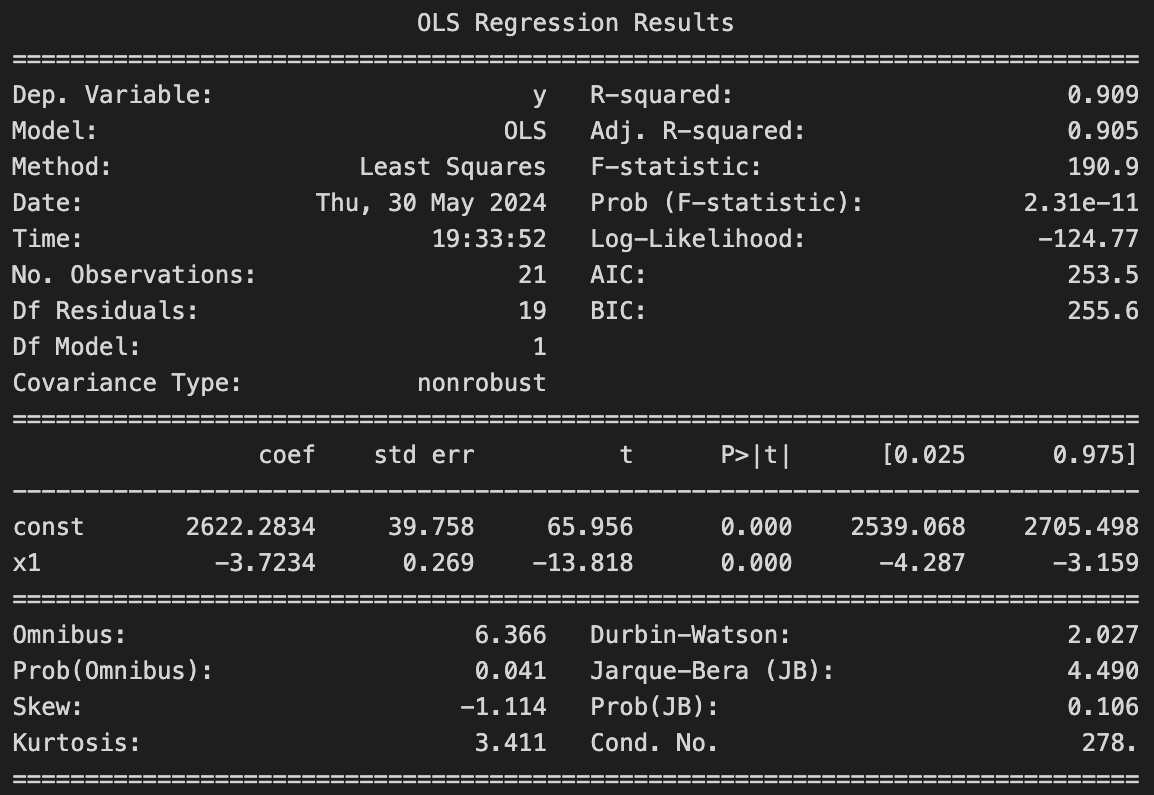
\includegraphics[width=0.8\textwidth]{figuras/fig20a}
        \caption{Descripci�n de la imagen.}
    \end{figure}
\end{frame}

\end{document}
